\documentclass{beamer}
\usepackage{graphics}
\title{Adding an accelerator to an AJIT processor system}
\author{Madhav P. Desai\\ Department of Electrical Engg.\\ IIT Bombay, Mumbai India}
\begin{document}
\maketitle



\frame[containsverbatim]{\frametitle{Overview}

\begin{itemize}
\item Adding an accelerator to an AJIT system is easy.
\item We assume that
\begin{itemize}
\item The accelerator has a slave programming interface for
configuration and monitoring.
\item The accelerator has a master memory interface to memory
shared with the processor.
\item The accelerator generates an interrupt to the processor.
\end{itemize}
\end{itemize}
}

\frame[containsverbatim]{\frametitle{Our example accelerator}

\begin{itemize}
\item The processor provides a 128 bit key to the accelerator.
\item The processor indicates the region of memory to
process.
\item The processor indicates to the accelerator that it
shall start processing.
\item On starting, the  accelerator computes an XOR of the key with 128-bit
blocks in the region of memory specified by the processor.
\item After finishing the job, the accelerator interrupts the processor.
\item The processor should service the interrupt and move on.
\end{itemize}

}

\frame[containsverbatim]{\frametitle{Steps}
\begin{itemize}
\item Fix the accelerator slave registers which can be controlled by
the processor via the slave interface.
\begin{itemize}
\item We use 16 32-bit registers, with register 0 mapped to address
0xffff4000.  See README for register map.
\end{itemize}
\item Implement the accelerator.
\begin{itemize}
\item We do this using AHIR (Aa to VHDL).
\item Verify the accelerator using simulation.
\end{itemize}
\item Integrate the accelerator with the processor to generate
an FPGA top-level description.
\item Synthesize.
\item Write a test example to confirm the processor accelerator
collaboration.
\end{itemize}
}

\frame[containsverbatim]{\frametitle{Integration of the accelerator with the processor}

\begin{figure}
  \centering
  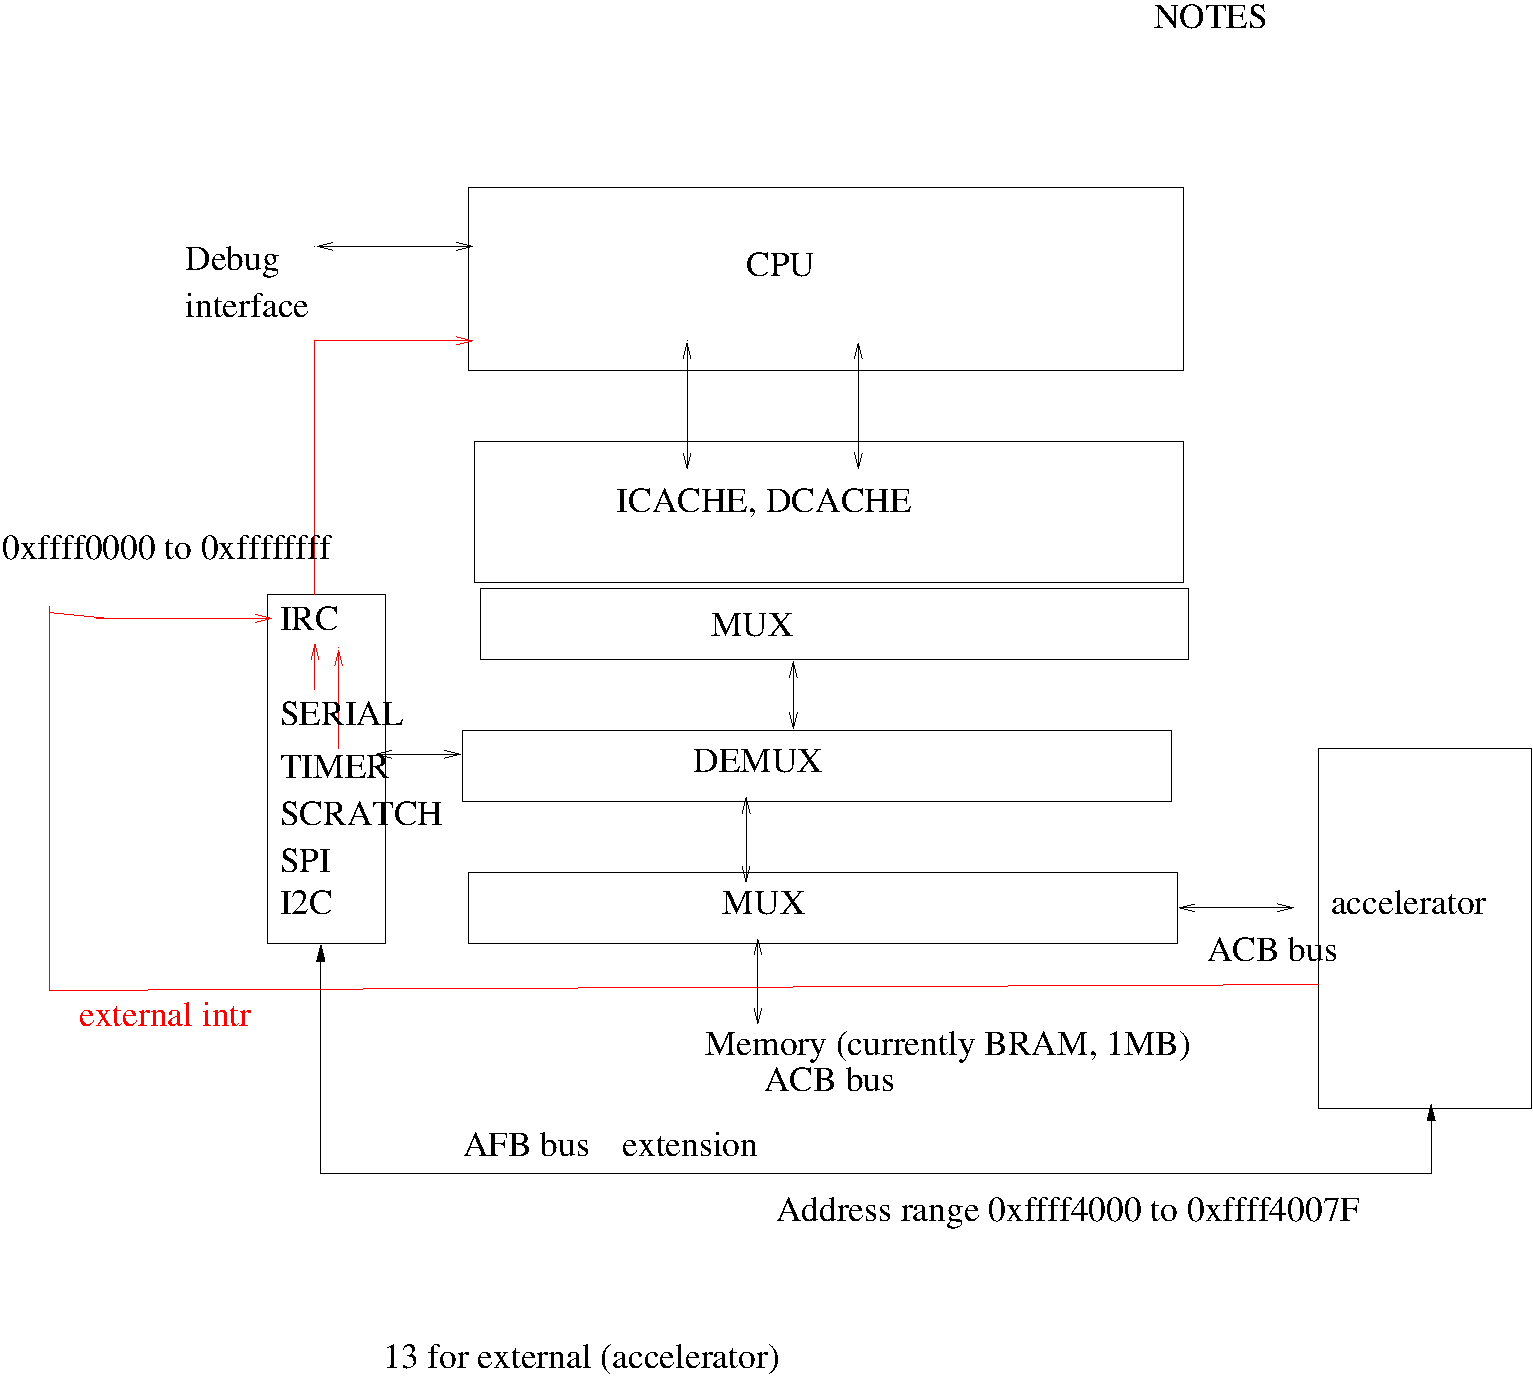
\includegraphics[width=10cm]{lite_with_accel.pdf}
  \caption{Overall system diagram}
\end{figure}

}

\frame[containsverbatim]{\frametitle{Demo}
\begin{itemize}
\item Take a look at the accelerator implementation in Aa.
\item The VHDL simulation of the accelerator (generated by Aa to VHDL).
\item The FPGA top-level.
\item The synthesis script.
\item The C test program for the processor, for checking the
accelerator.  Special attention to the interrupt handler.
\item Run it all and check!
\end{itemize}
}

\frame[containsverbatim]{\frametitle{Summary}
\begin{itemize}
\item End to end accelerator development flow.
\item Accelerator interfaces: slave to processor, master to memory, interrupt.
\item Easy to integrate: focus on accelerator implementation!
\end{itemize}

}



\end{document}
